%option->configure texmaker->edit-> lato medium 16
\documentclass[12pt]{article}
\usepackage{amsmath}

\usepackage{indentfirst}
\usepackage[font=scriptsize]{caption}
%\usepackage[font=small]{caption}10
%\usepackage[font=footnotesize]{caption}%9
%\usepackage[font=scriptsize]{caption}%8

\usepackage[utf8]{inputenc}
\usepackage{graphicx}
\usepackage{hyperref}
\usepackage[letterpaper,margin=0.75in]{geometry}
\usepackage{setspace}
\usepackage{comment}
\usepackage{amsmath}
\usepackage{esint}
\usepackage{wrapfig}
\usepackage{lipsum}
\usepackage{subcaption}
\usepackage{caption}

\begin{document}

\doublespacing


\begin{center}
{\Large \textbf{Developments of a Simple Model to Elucidate the Shape of Enveloped Viruses: Motivated by Monkeypox and SARS-CoV-2}}\\[1.5ex]
{\normalsize  Hua Deng}\\

{\normalsize February 21, 2025}
\end{center}





\begin{flushleft}
\setlength{\parindent}{30pt}
\section*{Specific aim}

\begin{comment}
--------------------------------------
First, to develop new models and simulations to study how the viral genome architecture(its shape, length and flexibility) influences the membrane. By combining polymer physics and liquid-state physics, such as crowding effects, we hope to gain a deeper understanding of viral assembly. By simulating how viral genomes behave in confined environments, we can uncover key principles behind virus formation and stability. It could contribute to more effective strategies for prevention and treatment of viral infections, especially for viruses like Monkeypox and SARS-CoV-2.


Second, studying the pressure inside viruses helps us better understand how viral genomes infect host cells and spread disease. It will be a different project to study the infectious process. When a virus packages its genetic material into its capsid/membrane, it builds up a lot of internal pressure. This pressure is key to initiate how viruses inject their DNA or RNA into host cells quickly and efficiently. By studying this process, we can uncover new ways to block viruses from replicating, such as targeting the proteins responsible for genome packaging, which could reduce internal pressure and prevent successful infection. It can inspire new drug delivery systems that work like viruses, help design better and more stable vaccines, and teach us more about the physical limits of DNA/RNA in extreme conditions.
----------------------------------
\end{comment}


First, our goal is to develop models and simulations combining polymer and liquid-state physics to study how viral genome properties—shape, length, and flexibility—influence membrane morphology. By simulating genome behavior in confined spaces, we seek to uncover key principles of viral assembly and stability, informing strategies to prevent and treat infections like Monkeypox and SARS-CoV-2.

Second, understanding internal pressure in viruses reveals how they inject their genomes into host cells. Packaging builds up pressure that drives rapid genome release. Studying this process may lead to antiviral strategies targeting genome packaging, inspire virus-like drug delivery systems, improve vaccine design, and deepen our understanding of nucleic acids under extreme confinement.
\vspace{-1em} 
\section*{Motivation}
\begin{comment}
------------------------------------------
In previous study, we developed a simple but still insightful model to investigate how monomers can self-organize into dimers, trimers, and tetramers on spherical surfaces, inspired by the trimeric spike proteins found in viruses like COVID-19. Using Monte Carlo simulations with attractive Yukawa potentials that include both radial and angular dependencies, we showed that trimers form more easily and are generally more stable than dimers. Tetramers, in contrast, require stronger attractive forces to form and are prone to aggregation when those forces become too strong. Analyses of energy and entropy contributions revealed that trimers are often more stable than dimers and, under certain conditions, as stable as tetramers. These findings are consistent with structural observations from cryo-electron microscopy studies of SARS-CoV-2 spike proteins, which show that trimers dominate the virion surface architecture\cite{Ke2020}. 

Beyond virus-related modeling, the researchers also explored how rod-like molecules
behave inside confined spaces, such as droplets or cavities, under molecular crowding. Our simulations showed that shorter rods tend to accumulate near the boundary, while longer rods align toward the center, consistent with experimental observations. These results emphasize the important role of both energetic and entropic factors in determining molecular organization in confined systems.

\begin{figure}[!ht]
  \centering
   \includegraphics[width=0.8\textwidth,height=5.5cm]{F-actin.png}
 
  \caption{\textbf{Left image:} Short DNA rods distribute near wall under molecular crowding. Long F-actin rods distribute in cavity interior and show high orientation ordering. Long F-actin rods distribute in cavity interior and show high orientation ordering.  Specific localization of 
  long DNA ($\lambda$ DNA) and F-actin in DEX-rich CAMDs.    
       \textbf{Right image:} Fluorescence microscopic images of DNA (GelGreen), actin (Alexa Fluor 546), and merged views are shown, along with polarization microscopy observations (four panels on the left). 
        The images were captured under the conditions of 120~$\mu$M $\lambda$ DNA, 10~$\mu$M actin, and 4.0~mM KCl. 
        F-actins were observed to be in a nematic liquid-crystal state at the center of DEX-rich CAMDs, while DNA molecules appeared segregated from the center. 
        In other words, long DNA strands are compressed by the aligned F-actin region, as schematically illustrated in the right panel. 
        Scale bar: 100~$\mu$m.\cite {nakatani2018}}
        %}
\end{figure}




We have successfully simulated the membrane along with the spike protein on its outer surface. We are now shifting our focus from the exterior to the interior of the membrane, concentrating on the interactions between the membrane and the enclosed genome. 
The goal is to better understand how viruses are organized, how the membrane and genome affect each other’s fluctuations, and how the genome is eventually released—insights that could help develop new antiviral treatments.
------------------------------------------------------------------------
\end{comment}




Previously, we investigated how spherical monomers self-organize into dimers, trimers, and tetramers on spherical surfaces, inspired by the trimeric spike proteins found in COVID-19 viruses. Using Monte Carlo simulations with an anistropic attraction and excluded volume repulsion between monomers, we identified the conditions that trimer formation becomes a favorable process. Both interaction energy form and interaction strength are crucial to surpass the entropically favorable dimers.  By adjusting the angular part of the anistropic interaction, tetramers become the major specie. The simulated trimers are consistent with structural observations from cryo-electron microscopy studies of SARS-CoV-2 spike proteins\cite{Ke2020}. 


Building on the foundation of our previous studies, we intend to develop a simple coarse-grained model with minimal parameters to elucidate how the interplay between the membrane and the enclosed genome regulates the shape of enveloped viruses. The goal of this approach is to provide deeper thermodynamic insights into viral interior organization above molecular length scales, the mutual influence between the membrane and genome, and the internal pressure created by viral genetic materials —knowledge that could inform the development of new antiviral strategies.

\begin{figure}[!ht]
  \centering
  \includegraphics[width=0.8\textwidth,height=4cm]{spike.trimer.png}
  \caption{Left image: Simulation of the SARS-CoV-2 spike protein on a spherical surface, illustrating the progression from randomly distributed monomers (left) to trimer (center) and tetramer (right) formations. Right image: SARS-CoV-2 for Covid-19 schematic image ( CDC Public
Health Image Library) \cite{cdc-covid}}
\end{figure}

\vspace{-1em} 
\section*{Background and Significance}
\begin{comment}
------------------------------------
Viral infections have a critical impact on global health, emphasizing their role in pandemics and outbreaks. These infections pose significant risks to public health and encompass a wide range of diseases, from seasonal influenza to more severe infectious diseases such as Monkeypox and COVID-19. Both Monkeypox and COVID-19 viruses are classified as enveloped viruses, which are distinguished by their lipid membranes that surround and protect their genomes. These membranes serve several crucial functions: they provide protection by shielding the viral genome from environmental factors and potential damage, and they facilitate transmission by enabling the virus to enter host cells. The membrane plays a key role in this process by interacting with specific receptors on host cells, thereby promoting viral infection and the delivery of the genome into the host. We need to further understand these mechanisms to develop effective prevention and treatment strategies.



Virions are acellular, meaning they are not made up of cells and therefore lack cellular components like organelles, ribosomes, or a plasma membrane. 


To elucidate the shape of enveloped viruses, one essential factor is on their genomes. The genome of a Monkeypox virus constitutes of a double stranded DNA of about 190 kb (kilo-bases) or 95 kbp (kilo-base pairs), that is 3000 nm in contour length, compared to the dimension of a virus particle at around 250 nm long\cite{erez2019diagnosis}\cite{parker2007human}. In Figure 3, the virus particles show spherical and oval shape, corresponding to immature and mature viruses, respectively.
------------------------------
\end{comment}

Viral infections significantly impact global health, driving pandemics and outbreaks. Enveloped viruses like Monkeypox and COVID-19 are surrounded by lipid membranes that protect their genomes and enable infection by interacting with host cell receptors. Understanding these mechanisms is key to developing effective treatments.

Virions are acellular particles lacking cellular structures such as organelles or membranes.
The shape of enveloped viruses is influenced by their genomes. Monkeypox virus has a ~190 kb double-stranded DNA genome (~3000 nm contour length), much larger than the ~250 nm virus particle \cite{erez2019diagnosis}\cite{parker2007human}. As shown in Figure 2, immature viruses are spherical, while mature forms appear oval.
This study investigates how genome shape influences membrane morphology in virus particles, focusing on the transition from spherical (immature) to oval (mature) forms. Using a coarse-grained model and Monte Carlo simulations, we will examine how genome compaction, fluctuations, and spatial arrangement drive membrane deformation during virus maturation.




\begin{figure}[!ht]
  \centering  
  \fbox{\includegraphics[width=0.4\textwidth,height=4cm]{electron.monkeypox.png}}
  \caption{Electron microscopic (EM) image for
Monkeypox virus particles. Oval-shaped
virus particles are mature, and spherical
particles are immature virions \cite{goldsmith2003monkeypox}}
\end{figure}


\begin{comment}
-------------------------------------------
The goal is to investigate the relationship between genome shape and membrane morphology in virus particles, focusing on the transition from spherical to oval geometries. Spherical shapes are typically associated with immature viruses, while mature viruses tend to exhibit more elongated, oval forms. By using a coarse-grained model and Monte Carlo simulations, we will explore how changes in the genome configuration—such as compaction, fluctuation, or spatial arrangement—affect the deformation and final shape of the surrounding lipid membrane. This study will help elucidate how the shape of the genome affects membrane curvature during virus maturation.





In contrast to Monkeypox viruses, SARS-CoV-2, the virus responsible for COVID-19, are spherical and their diameter is around 80-120 nm, much smaller than the size of a Monkeypox virion. In terms of
their genomes, Covid-19 viruses belong to the family of
RNA viruses as common corona flu viruses. Unlike
seasonal flu viruses, the Covid-19 virus has the longest
RNA among known corona viruses, consisting of a single
~30 kb strand of RNA with a contour length at about
1,400 nm. \cite{baron2020sars}\cite{Wu2022}


SARS-CoV-2 enters a host cell by first using its spike (S) protein to bind to a specific receptor on the surface of human cells called ACE2 (angiotensin-converting enzyme 2). This spike protein acts like a key, allowing the virus to attach tightly to the host cell. After attachment, the virus enters the cell either through direct fusion with the cell membrane or via endocytosis.\cite{Barrow2013}\cite{payne2022viruses} When a virus infects a host, it deliberately breaks this symmetry. Doing so creates weaker areas on the surface of the capsid, which then open up to allow the virus to inject its genetic material (RNA or DNA) into the host cell. In this way, breaking symmetry is an essential part of the infection mechanism.
------------------------------------
\end{comment}






In contrast, SARS-CoV-2 particles are smaller (~80–120 nm) and spherical, with a single ~30 kb RNA genome (~1,400 nm contour length) \cite{baron2020sars}\cite{Wu2022}. SARS-CoV-2 infects host cells by binding its spike (S) protein to the ACE2 receptor, facilitating entry through membrane fusion or endocytosis \cite{Barrow2013}\cite{payne2022viruses}. During infection, the virus breaks capsid symmetry to create weak spots that allow genome release, a crucial step in initiating infection.

\begin{figure}[htbp]
  \centering
  \begin{subfigure}[t]{0.45\textwidth}
    \centering
    \vtop{\null
      \hbox{\fbox{\includegraphics[width=\linewidth,height=4.5cm]{endocytosis.png}}}
      \caption{Illustration of the steps of virus entry via clathrin-mediated endocytosis. (A) Virus approaches the cell surface. (B) Biochemical interactions between ligands and receptors attract virus to the cell surface. (C) Virus attaches to the cell surface and signals the cell. (D) A clathrin-coated pit is formed around the bound virus. (E) A clathrin-coated vesicle is formed, and the dynamin at the neck region facilitates vesicle scission. (F) The vesicle travels to the cell interior \cite{Barrow2013}.}
      \label{fig:endocytosis}
    }
  \end{subfigure}
  \hfill
  \begin{subfigure}[t]{0.45\textwidth}
    \centering
    \vtop{\null
      \hbox{\fbox{\includegraphics[width=\linewidth,height=4.5cm]{fusion.png}}}
      \caption{Membrane fusion. Many viruses, both enveloped and unenveloped, are brought into cells by endocytosis. The low pH environment in the endosome triggers molecular rearrangements of capsid or envelope proteins. In this example, an enveloped virus is fusing with an endosomal membrane to release the capsid into the cytosol \cite{payne2022viruses}.}
      \label{fig:fusion}
    }
  \end{subfigure}

  \caption{Comparison of virus entry mechanisms: (a) Clathrin-mediated endocytosis, and (b) Membrane fusion.}
  \label{fig:sidebyside}
\end{figure}


Once inside, the viral envelope is removed (a process called uncoating), releasing its positive-sense single-stranded RNA genome into the host cell’s cytoplasm. This viral positive-sense single-stranded RNA acts directly as messenger RNA (mRNA) and is translated by the host's ribosomes to produce viral proteins, including more spike proteins, structural proteins, and enzymes necessary for viral replication. The viral genome is also copied to make more RNA strands. These components are then assembled into new viral particles. Finally, the new viruses are released from the cell by budding, often taking a piece of the host’s membrane with embedded spike proteins, allowing them to infect new cells. The spike protein is essential for both the entry of the virus and for determining which cells it can infect.
 
Unlike Monkeypox virus, which transitions from spherical to oval shapes, SARS-CoV-2 remains spherical throughout its life cycle. However, this study explores whether similar physical principles apply. By adjusting genome length, membrane size and membrane shape in coarse-grained models and Monte Carlo simulations to match SARS-CoV-2 dimensions, our goal is to examine how genome compaction, fluctuations, and arrangement influence membrane deformation. This approach may uncover general physical constraints on genome–membrane interactions that impact viral assembly and stability across different viruses.

%------------------------------------------------------------------------------------------------------------------

A related but distinct question is how viruses build and release internal pressure to inject their genomes into host cells. 
Viruses pack their DNA or RNA into capsids or membranes under extremely high pressure, often tens of atmosphere. During assembly, ATP-powered motor proteins force the genome into the confined capsid space, requiring significant energy. This tight packing generates high internal pressure due to two main factors: electrostatic repulsion between negatively charged nucleic acid strands and the bending strain of compressing a long, rigid molecule into a much smaller space than its relaxed form\cite{BrandarizNunez2019}.

This pressurization plays a crucial role in infection. When the virus contacts a host cell, the stored pressure acts like a compressed spring, rapidly ejecting the genome into the host. This fast genome release allows the virus to hijack the host’s machinery almost immediately. Such pressure-driven ejection is conserved across many viral families, including herpes simplex virus type 1 (HSV-1), which builds up to 20 atmospheres of pressure.

To understand this mechanism, we will use coarse-grained models and Monte Carlo simulations to study how genome packing and membrane or capsid deformation together generate internal forces. By exploring how genome arrangement and structural properties regulate pressurization, our goal is to identify potential antiviral targets that block pressure-driven genome ejection, offering new strategies to prevent infection.






\vspace{-2em} 
\section*{Research Plan}
\vspace{-1em}
\subsection*{I. Techniques}
\vspace{-1em}
 \subsection*{\indent{1. Coarse-Grained Modeling (CGM)}}
\begin{tabbing}
\indent\indent	(1) \= Simplifies complex systems by grouping atoms/molecules into larger particles (beads).\\
\indent\indent	(2) \> Enables large-scale simulations with reduced computational cost.
\end{tabbing}



\subsection* {\indent {2. Continuum Mechanics}}
\begin{tabbing}
 \indent \indent    (1) Treats membranes as continuous, deformable surfaces.\\

 \indent  \indent   (2) Describes large-scale membrane behavior using differential geometry and energy functionals.\\

\indent  \indent (3) Statistical Physics (Boltzmnn Distribution, Ensembles).\\

 \indent  \indent    (4) Governs the probability of system states based on temperature and energy.\\

  \indent \indent  (5)   Used in defining acceptance rules and thermodynamic constraints (NVT/NPT).
\end{tabbing}


\begin{figure}[!ht]
  \centering
  \fbox{\includegraphics[width=0.75\textwidth,height=5cm]{discrete.png} }
  \caption{Different computational methods developed to study cellular membranes are valid in different length and time scales.\cite{chabanon2017systems}}
\end{figure}


\subsection*{\indent{3. Monte Carlo Simulation (MC)}}
\begin{tabbing}

  \indent\indent    (1) Stochastic method to explore system configurations based on energy-driven probability.\\

    \indent\indent (2) Especially useful in equilibrium or thermodynamic studies without tracking real-time dynamics.
\end{tabbing}



\subsection*{II. Procedure and Methods} 


These are the specific models and procedures implemented using the above techniques.\\


  \subsection*{\indent{ 1. Kremer–Grest Bead-Spring Model}}

     \indent\indent  (1)For genome (DNA/RNA) representation.

      \indent\indent (2) Uses:

         \indent\indent \indent (1) FENE potential for bonded interactions.

          \indent\indent \indent   (2) WCA potential for excluded volume (non-bonded interactions).

  \subsection*{\indent{2. Helfrich–Canham Membrane Model}}

  	 \indent\indent(1)Describes membrane bending energy:

\vspace{-1em}
\begin{align}
F_\text{full mem} = \int_S \Bigg[
&\underbrace{\frac{\kappa}{2} \left(2H - C_0(\vec{r}) \right)^2}_{(1)\ \text{spontaneous-curvature-modified bending}} 
\ + \ 
\underbrace{\bar{\kappa} K}_{(2)\ \text{Gaussian-curvature term}} 
\Bigg] dA \nonumber \\
&\quad + \ 
\underbrace{\lambda A}_{(3)\ \text{area constraint}} 
\ + \ 
\underbrace{p V}_{(4)\ \text{volume constraint}}.
\end{align}

\indent\indent (2)Discrete angle-based version used for simulations.

\begin{equation}
E_{\text{bend}} = \kappa \sum_{\langle i,j \rangle} \left(1 - \cos \theta_{ij} \right)
\end{equation}


\subsection*{\indent{3. Monte Carlo Move Set}}

    \indent\indent(1)Randomly displace particles (DNA beads, crowders, or membrane vertices).

   \indent\indent(2) Accept/reject moves using:\\
  \indent\indent\indent Metropolis criterion:
%\setlength{\parindent}{0pt}
\begin{equation}
P_{\text{accept}} = \min \left(1, e^{-\beta \Delta E}\right)
\end{equation}

    
  \subsection*{\indent{ 4. Excluded Volume Implementation}}

   \indent\indent Prevents overlap of DNA beads and crowders using WCA or Lennard-Jones (LJ) potentials.
   
   Excluded volume is an essential aspect of Coarse rained (CG) modeling, ensuring that two particles do not occupy the same space. Without it, particles in a simulation may overlap or penetrate each other, leading to unphysical results. To account for excluded volume, repulsive interaction potentials—such as the Lennard-Jones potential or its softer variants used in models like MARTINI or DPD—are applied. These potentials create a repulsive force that prevents particles from getting too close. Key parameters like bead size ($\sigma$) and interaction strength ($\varepsilon$) must be carefully tuned to reflect the physical size and behavior of the particles.

Before running a simulation, energy minimization and equilibration steps are typically used to eliminate any initial overlaps and ensure a stable starting configuration. Properly enforcing excluded volume is particularly important in biomolecular and polymer systems, where structural integrity and thermodynamic behavior depend on particles keeping natural distances and not overlapping unrealistically. Ignoring or mishandling excluded volume can compromise the accuracy and reliability of the simulation.


\subsection*{\indent{5. Simple Liquid Models}}

   \indent\indent Used for simulating crowders around DNA:

       \indent\indent (1)Hard Sphere model: purely repulsive.

      \indent\indent (2)Lennard-Jones model: includes both attraction and repulsion.
      
      
Simple liquid models that help understand the structure and behavior of polymer in crowded environments. Specifically, the simple liquid models referenced include Hard Sphere Model and Lennard-Jones Model. 

Hard sphere model is used to understand the behavior of particles in crowded environments, where the excluded volume effect becomes important. 

The Lennard-Jones model accounts for both attractive and repulsive forces between particles, which is important in understanding the interactions within fluids and condensed matter. It helps model the behavior of molecules, especially in non-ideal conditions like those found in crowded environments. 

\subsection*{\indent{6. Ensemble Settings}}
Simulations are run under NPT and NVT ensembles to explore equilibrium states and fluctuations.

(1) NVT (Canonical Ensemble): Constant number of beads, volume, and temperature.
   
  

\indent\indent NVT stands for:

 \indent\indent\indent  N = Number of beads (constant)\\

 \indent\indent\indent  V = Volume (constant)\\

 \indent\indent\indent  T = Temperature (constant)

Under NVT conditions, the volume of the system is fixed, meaning the membrane is constrained and cannot expand or contract. In one approach, the membrane is initialized with an oval or ellipsoidal shape, defined by input parameters a, b, and c, representing the lengths along its three principal axes. These parameters remain constant throughout the simulation, so the membrane keeps its shape even as the genome inside moves or grows. Because the membrane cannot adapt naturally to changes, any pressure exerted by the genome builds up inside, sometimes leading to artificial forces that would not normally appear in a flexible system.

In another approach, even though the overall volume remains fixed under NVT, small local fluctuations in the shape of the membrane are allowed while still keeping a, b, and c centered around their initial values. In this case, the membrane can slightly deform in response to internal forces from the genome without changing its total volume. While the confinement effect is still strong, allowing limited local fluctuations provides a somewhat more realistic interaction between the genome and the membrane. Studying the membrane–genome relationship in either method under NVT is useful for early-stage stabilization or when specifically exploring how genomes behave in confined, rigid environments.

   
   
   
   

(2) NPT (Isothermal–Isobaric Ensemble): Constant number of beads, pressure, and \\
  \indent temperature, allowing volume fluctuations. Simulating realistic physical conditions, since 
  \indent many experiments happen at constant pressure (example:1 atm) and temperature  (example: 
  \indent 298 K).

NPT stands for:

  \indent\indent  N = Number of beads (constant)

  \indent\indent  P = Pressure (constant)

  \indent\indent  T = Temperature (constant)
    
    Under NPT conditions, the system’s pressure is controlled, allowing the volume to change naturally over time. In one approach, the membrane is initialized with a fixed oval or ellipsoidal shape, defined by the input parameters a, b, and c, which represent the lengths along its three principal axes. These parameters remain constant during the simulation, so the membrane maintains its overall shape while still allowing local fluctuations and interactions with the genome inside.

In another approach, the parameters a, b, and c are allowed to fluctuate during the simulation. This means the membrane can expand, shrink, or reshape dynamically in response to internal forces exerted by the genome. Such flexibility promotes more realistic interactions between the genome and the membrane — for example, the genome may push outward and deform the membrane, while changes in membrane tension or curvature can influence how the genome is organized. Using NPT conditions in this way provides a natural and dynamic view of the interplay between membranes and genomes in biological systems.
         
   

\subsection*{\indent{7. Pressure Calculation by Theoretical Model}}


Previous studies, such as Grayson et al.\cite{Grayson2006}, have described the packaging energy of DNA by modeling the capsid as a sphere and the genome as an extended semiflexible rod. In our work, we apply a similar approach: we represent the membrane as a spherical enclosure and the RNA as an extended semiflexible rod.

Our goal is to quantify how the structure of the genome influences the internal pressure within the membrane. Specifically, we aim to understand how changes in the RNA persistence length  \(\xi\)\ and the radial loop distribution \(N(r)\) affect the pressure \(P\) generated during packaging. This pressure arises primarily from the bending energy of the confined RNA. To estimate it, we divide the total bending energy of the RNA by the volume of the membrane. In this way, we link the physical properties of the RNA and its spatial organization directly to the internal pressure experienced by the membrane.   


\begin{equation}
P = \frac{\sqrt{3} k_B T \, \xi^2}{R^3} \int_{R_\text{in}}^{R_\text{out}} \frac{N(r)}{r} \, dr
\end{equation}



\subsection*{Simulation Procedures}
(1)Initialization of DNA chains and crowders.

(2) Energy calculation (FENE + WCA/LJ).

(3) Repeated Monte Carlo updates to reach equilibrium.

\subsection*{\indent{8. Pressure Calculation by Primitive Model}}
We use the Primitive Model (PM) to simulate the pressure exerted by the genome as it passes through a narrow slit in the membrane. Primitive Model (PM)	is a specific type of coarse-grained model that uses minimal physics (e.g., hard spheres + short-range bonding) to capture essential behavior.


 
In our research, the genome chain, represented as a series of beads connected by covalent bonds, translocates through a small slit in the membrane, and each bead is treated as a rigid, impenetrable sphere with a diameter $ \sigma $. The contact theorem\cite{Voertler1997} applies by relating the pressure normal to the slit walls, $ p_w $, to the one-particle density of these beads at the contact distance $ z = \sigma/2 $, expressed as 

\begin{equation}
p_w = \rho_{\left(z = \frac{\sigma}{2}\right)} k_B T
\end{equation}

\subsection*{Simulation Procedures}

(1)Genome modeled as hard spheres (Primitive Model).

(2)Confined in a slit geometry.

(3)Simulate genome movement and collisions.

(4)Measure bead density at wall contact.

(5)Compute pressure using contact theorem
\subsection*{III. Hypothesis}
\noindent \textbf{Hypothesis 1:}\\
The shape of a virus forms after its genome architecture stabilizes. First, the genome reaches a steady state, and we then examine how it influences the viral membrane shape. 

\noindent \textbf{Hypothesis 2:}\\
The genome architecture may develop after the viral membrane shape stabilizes. In this case, the membrane reaches a steady state first, and we then observe how it affects the genome’s geometry. By adjusting the length of 1D rod or the perimeter of the circle of the genome, we try to match the reference.\cite{goldsmith2003monkeypox}\\

\noindent \textbf{Hypothesis 3}:\\
The shape of a virus and its genome architecture form simultaneously.
The model for this hypothesis allows both genome morphology and membrane shape to undergo simultaneous
fluctuation until both arrive at a mutual steady state.

	
\noindent \textbf{Hypothesis 4:}\\
In a Monte Carlo simulation of a genome confined within a sealed membrane or slit-like pore, different theoretical and computational methods for calculating pressure—such as those based on the primitive model (PM) and theoretical model—should yield consistent values for the normal pressure on the membrane walls, provided that the simulation is correctly implemented and the system is properly equilibrated.




\subsection*{IV.Expected outcomes} 
%\subsection*{IV.Possible pitfalls} 
(1)The shape of a virus and its genome architecture form simultaneously.
	
\begin{figure}[!ht]
  \centering
  \fbox{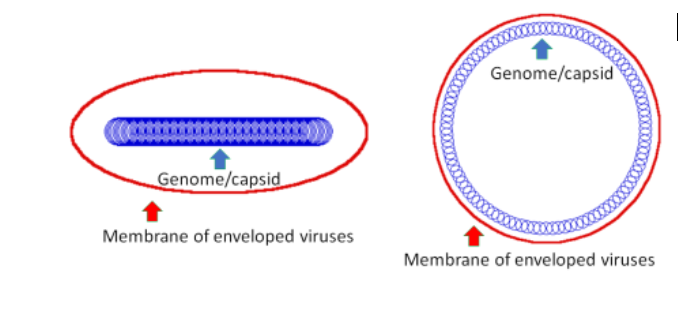
\includegraphics[width=0.5\textwidth,height=3.7cm]{monkeypox.png}}  % Adjust width or height as needed
  \caption{Preliminary 2D model studies to
investigate the effect of the geometry of a
genome on the shape of a virus. A rod-like
genome induces an elliptic shape whereas a
circular genome leads to a circular shape.}
\end{figure}

(2)The expectation that different methods for calculating the pressure in a Monte Carlo simulation of a system, such as the primitive model (PM) of genome in slit-like pores should yield consistent values for the pressure normal to the walls of membrane, assuming the methods are correctly implemented and the system is properly equilibrated.

\subsection*{V.Projected timeline}

Months 0-3: Fine-tune the continuum membrane model.\\
Months 4-6: Investigate competition among different membrane shapes.\\
Months 7-9: Study chain model and crowding effect\\
Months 10-12:Expand the developed models from 2D to 3D.\\


\newpage

\end{flushleft}
\bibliographystyle{unsrt}
\bibliography {references}  

\end{document}




